\documentclass[border=6pt]{standalone}
\usepackage[T1]{fontenc}
\usepackage[utf8]{inputenc}
\usepackage[scaled=0.98]{helvet}
\renewcommand{\familydefault}{\sfdefault}
\usepackage{amsmath}
\usepackage{graphicx}
\graphicspath{{../../../../../../exercises_lecturenotes/lecture_notes/kurs100_lektionsnoter/}}
\usepackage{tikz}
\usepackage{pgfplots}
\pgfplotsset{compat=1.18}
\usetikzlibrary{arrows.meta, decorations.pathreplacing, calc, positioning, fit, backgrounds, shapes.geometric}
\usepgfplotslibrary{groupplots,fillbetween}
\definecolor{scanpink}{HTML}{E5006D}
\definecolor{scanteal}{HTML}{00A6A6}
\definecolor{scannavy}{HTML}{243746}
\definecolor{scanlightgray}{HTML}{F1F2F3}
\begin{document}
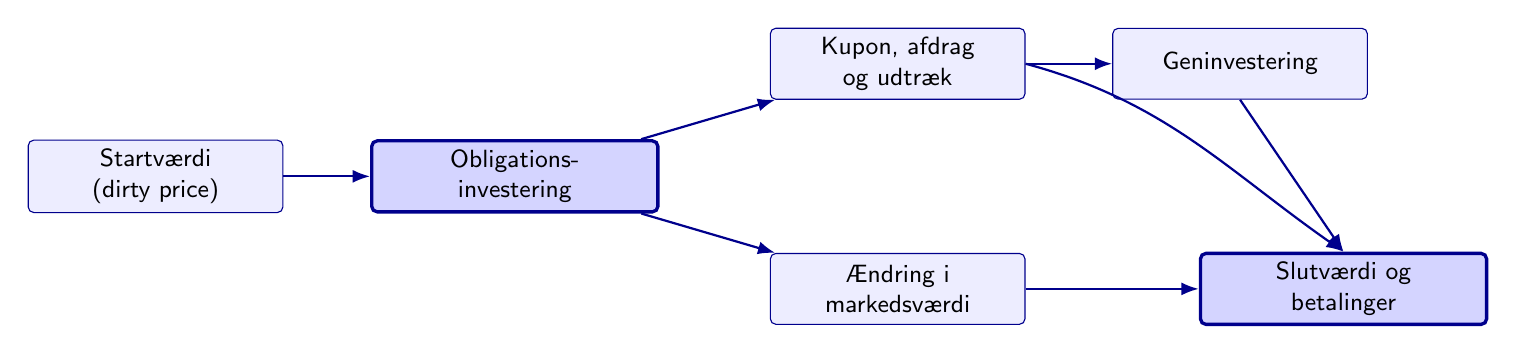
\begin{tikzpicture}[
    node distance=8mm and 11mm,
    flow/.style={draw=blue!55!black, rounded corners=2pt, fill=blue!7,
        align=center, minimum height=9mm, text width=30mm, font=\small},
    core/.style={flow, fill=blue!17, very thick, text width=34mm},
    arrow/.style={-{Latex[length=2.2mm]}, thick, draw=blue!55!black}
]
\node[flow] (start) {Startværdi\\(dirty price)};
\node[core, right=of start] (bond) {Obligations-\\investering};
\node[flow, above right=5mm and 14mm of bond] (payments) {Kupon, afdrag\\og udtræk};
\node[flow, below right=5mm and 14mm of bond] (market) {Ændring i\\markedsværdi};
\node[flow, right=of payments] (reinvest) {Geninvestering};
\node[core, right=22mm of market] (end) {Slutværdi og\\betalinger};
\draw[arrow] (start) -- (bond);
\draw[arrow] (bond) -- (payments);
\draw[arrow] (bond) -- (market);
\draw[arrow] (payments) -- (reinvest);
\draw[arrow] (payments.east) to[out=-15,in=145] (end.north);
\draw[arrow] (reinvest.south) -- (end.north);
\draw[arrow] (market) -- (end);
\end{tikzpicture}
\end{document}
